\chapter{Introducción}

\section{Descripción del problema}

La \textbf{antropología forense} (\textbf{AF}) es un subcampo de la antropología\footnote{La antropología (del griego ánthrōpos, «hombre (humano)», y logos, «conocimiento») es la ciencia que estudia al ser humano de una forma integral, de sus características físicas como animales y de su cultura.}, concretamente de la antropología física\footnote{La antropología biológica o antropología física es una rama de la antropología y la biología que tiene como objeto el estudio de la evolución y variabilidad biológica humana, tanto pasada como actual.}, que aborda el análisis de restos óseos humanos de importancia médica y legal \cite{ubelaker2008forensic}. Los expertos en dicha disciplina, dado su conocimiento de la biología del esqueleto humano y materias relacionadas, examinan los huesos humanos con el objetivo de obtener la mayor cantidad de información posible sobre las personas representadas por los restos óseos.\\

% El siguiente párrafo podría modificarse y cambiarse por los dos objetivos principales según \cite{ubelaker2008forensic}:
% - Asistir en la identificación de restos humanos y en la interpretación de sus circunstancias.

Los antropólogos forenses tratan de cumplir con cinco objetivos principales a la hora de realizar su trabajo \cite{byers2016introduction}:
\begin{itemize}
    \item Determinar el grupo poblacional, sexo, edad y estatura de la persona a la que pertenecen los restos óseos estudiados una vez los tejidos blandos se han deteriorado hasta tal punto que no es posible determinarlos mediante análisis visual.
    \item Cuando hay evidencia de heridas traumáticas en los restos óseos, identificar la naturaleza de estas heridas y sus posibles causas con la intención de recoger información para determinar la causa y circunstancias del fallecimiento.
    \item Establecer un intervalo \textit{postmortem}, la cantidad de tiempo que ha pasado desde que la persona objeto de estudio falleció.
    \item Asistir en la localización y recuperación de restos superficiales o enterrados, de manera que toda la evidencia correspondiente a la investigación forense sea recogida.
    \item Proveer información útil en la obtención de una identificación positiva de personas fallecidas.
\end{itemize}

Además de lo anteriormente mencionado, la AF cumple otras funciones dentro de la sociedad moderna. Se consulta a los especialistas en AF para la identificación de víctimas de catástrofes como accidentes aéreos, guerras, ataques terroristas o desastres naturales \cite{vallejo2009identificacion}. También asisten en el estudio de crímenes de guerra derivados de los numerosos arrestos de civiles producidos por la violencia política, particularmente en países de América central y del sur, África y Europa \cite{casallas2004antropologia}. Por último, también participan en la estudio de personas históricamente relevantes pero no relevantes desde el punto de vista médico y legal  \cite{byers2016introduction}.\\



De los objetivos de la AF citados con anterioridad, el que posee mayor relevancia para el desarrollo de este proyecto, es el campo de la \textbf{Identificación Humana} (\textbf{ID}) y \textbf{la estimación del perfil biológico} (\textbf{PB}). La AF proporciona una alternativa con un mayor rango de aplicabilidad que otras técnicas de ID como análisis de huellas dactilares o análisis de ADN. Esta ciencia contribuye a la identificación de restos humanos de dos maneras: proporciona métodos que establecen identificaciones positivas y métodos que contribuyen a la identificación limitando las potenciales coincidencias con el individuo analizado \cite{mesejo2020survey}. La AF entra en escena cuando la descomposición del tejido blando está tan avanzada que los médicos forenses especialistas no pueden determinar características como la demografía, el tiempo, la causa y las circunstancias del fallecimiento. Sin embargo, los antropólogos forenses se involucran cada vez más como consultores, incluso cuando existe tejido blando presente.\\

La estimación del \textbf{PB} tiene un papel crucial a la hora de reducir el rango de posibles coincidencias a la hora de identificar determinados restos óseos. En la Figura \ref{fig:skeletonpipeline} podemos ver que la estimación del PB es uno de los primeros pasos en el proceso de ID forense. El PB combina el estudio de los restos óseos con el objetivo de encontrar los rasgos característicos que determinan la identidad de un individuo. Entre estos rasgos característicos encontramos los siguientes:

\begin{itemize}
    \item Estimación del sexo en individuos adultos y subadultos (niños).
    \item Estimación de la edad en individuos adultos y subadultos vivos o fallecidos.
    \item Estimación de la altura mediante el uso de huesos largos.
    \item Estimación de la ascendencia.
\end{itemize}

\begin{figure}[ht!]
    \centering
    \includegraphics[width=\textwidth]{imagenes/skeletonpipeline.png}
    \caption[Diagrama de secuencia de los pasos realizados en la identificación forense basada en el esqueleto.]{Diagrama de secuencia de los pasos realizados en la identificación forense basada en el esqueleto (skeleton-based forensic identification, SFI) \cite{mesejo2020survey}.}
    \label{fig:skeletonpipeline}
\end{figure}

Para llevar a cabo la tarea de estimar de la edad de un individuo (o cadáver) existen numerosos métodos utilizados por los antropólogos forenses \cite{hanihara1978estimation}. Podemos clasificarlos en métodos dentales y esqueléticos según si analizan la dentadura o se centran en cualquier otro hueso del esqueleto humano. Dentro de los métodos que analizan los huesos, la estimación de la edad a partir de la observación de características macroscópicas en las sínfisis púbicas es uno de los enfoques más aceptados.\\

\begin{figure}[ht!]
    \centering
    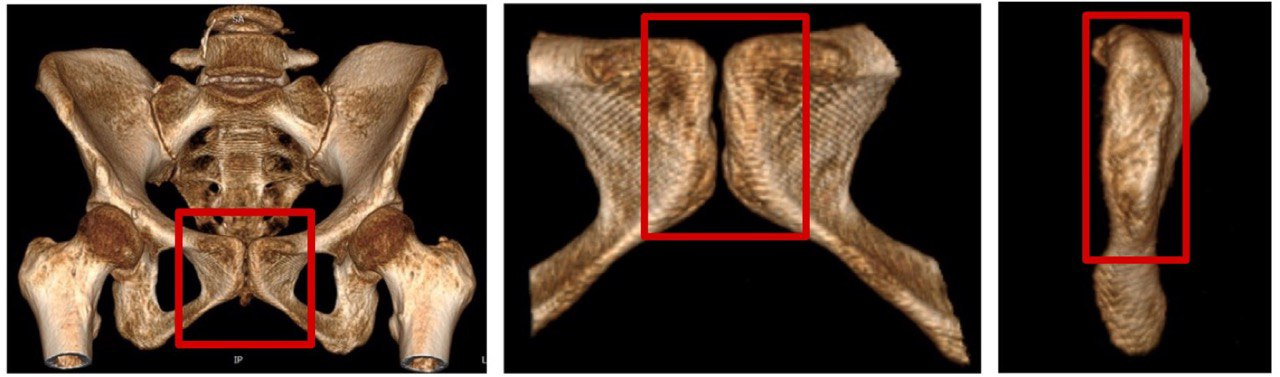
\includegraphics[width=\textwidth]{imagenes/pubis.jpg}
    \caption[Reconstrucción volumétrica por tomografía computerizada 3D de la sínfisis del pubis.]{Reconstrucción volumétrica por tomografía computerizada 3D de la sínfisis del pubis en RadiAnt \cite{hisham2019quantification}. Las imágenes no tienen la misma escala. \textbf{Izquierda}: Pelvis humana. \textbf{Centro}: Ampliación de ambas partes del pubis. \textbf{Derecha}: Cara del pubis izquierdo. Encuadrado en rojo se ha marcado la sínfisis púbica.}
    \label{fig:pubis}
\end{figure}

Como podemos apreciar en la Figura \ref{fig:pubis}, la sínfisis del pubis es la conexión entre las dos partes del pubis. Esta puede observarse tanto en la cara del pubis derecho como del izquierdo. Es en estas caras donde los antropólogos forenses centran su atención a la hora de identificar características morfológicas. Estas características, discriminatorias y observables a simple vista, fueron descritas por T. W. Todd en su artículo \textbf{\textit{Ages changes in the pubic bone}} (1921) \cite{todd1921age}. Aún a día de hoy, 100 años después de la publicación de este artículo, los antropólogos forenses localizan y emplean las características descritas por Todd a la hora de estimar la edad de los restos óseos de personas muertas en edad adulta. Entre dichas características se encuentran: la porosidad, definición y profundidad de las crestas y surcos; la porosidad y regularidad de la superficie y la presencia de nódulos o bordes; entre otras. En la Figura \ref{fig:toddfeatures} podemos ver un ejemplo de algunas de las características definidas por Todd.

\begin{figure}[ht!]
    \centering
    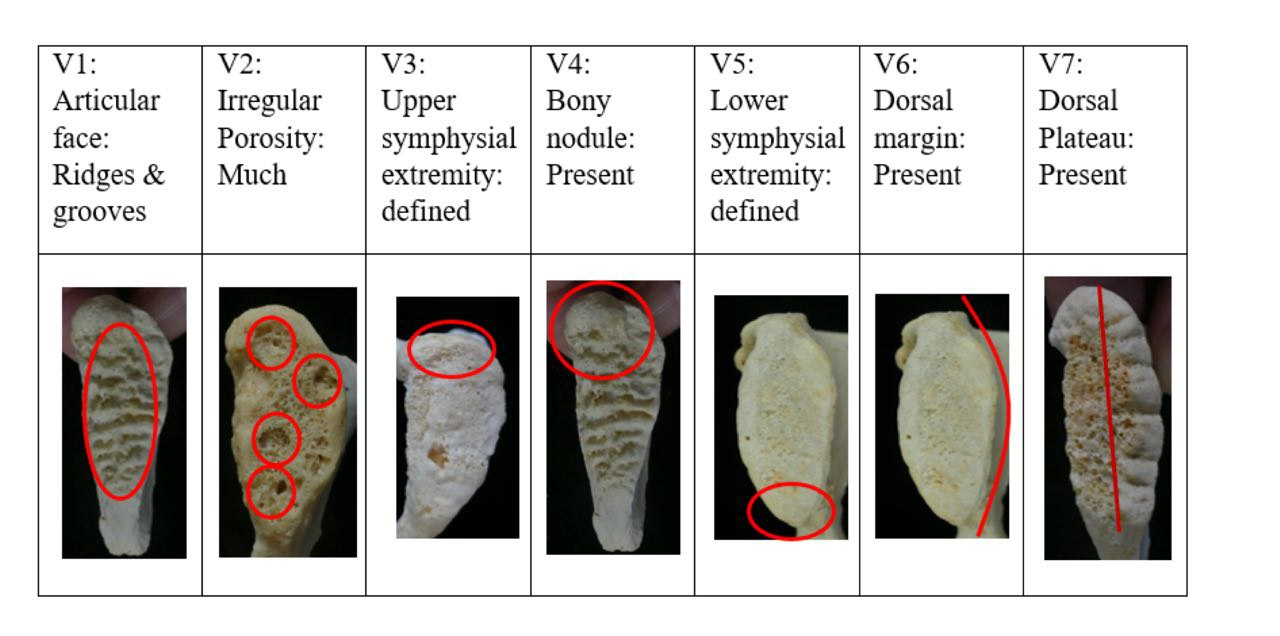
\includegraphics[width=\textwidth]{imagenes/Toddfeatures.jpg}
    \caption[Características morfológicas en la sínfisis púbica.]{Algunos ejemplos de características que definen el desarrollo típico y los cambios morfológicos degenerativos en la sínfisis púbica durante el crecimiento. Las regiones de interés están resaltadas en rojo}
    \label{fig:toddfeatures}
\end{figure}

Todd también estableció varios rangos de edad para los que los restos óseos presentaban características similares. Como se puede observar en la Tabla \ref{tab:rangosTodd} estos rangos o fases abarcan de 1 o 2 años para muestras jóvenes (18-26 años) a 4 años de diferencia en las últimas fases. Además el último rango de edad es catalogado como 50 años o más. Esto era adecuado para la época de publicación del artículo, pero queda bastante obsoleto en el momento actual en el que la esperanza de vida es superior.\\ 
% Estos rangos o fases son los siguientes:
% \begin{itemize}
%     \item Fase 1: 19 años
%     \item Fase 2: 20 a 21 años
%     \item Fase 3: 22 a 24 años
%     \item Fase 4: 25 a 26 años
%     \item Fase 5: 27 a 30 años
%     \item Fase 6: 31 a 34 años
%     \item Fase 7: 35 a 39 años
%     \item Fase 8: 40 a 44 años
%     \item Fase 9: 45 a 49 años
%     \item Fase 10: 50 años o más
% \end{itemize}


% % Please add the following required packages to your document preamble:
% % \usepackage{graphicx}
% \begin{table}[ht!]
% \centering
% \begin{tabular}{|l|l|}
% Fase 1 & 19 años \\
% Fase 2 & 20 a 21 años \\
% Fase 3 & 22 a 24 años \\
% Fase 4 & 25 a 26 años \\
% Fase 5 & 27 a 30 años \\
% Fase 6 & 31 a 34 años \\
% Fase 7 & 35 a 39 años \\
% Fase 8 & 40 a 44 años \\
% Fase 9 & 45 a 49 años \\
% Fase 10 & 50 años o más
% \end{tabular}%
% \caption{Intervalos de edad de la muerte propuestos por Todd.}
% \label{tab:rangosTodd}
% \end{table}

% Please add the following required packages to your document preamble:
% \usepackage{graphicx}
\begin{table}[ht!]
\centering
\begin{tabular}{|l|l|l|l|}
\hline
\textbf{Fase 1} & 19 años & \textbf{Fase 6} & 31 a 34 años \\ \hline
\textbf{Fase 2} & 20 a 21 años & \textbf{Fase 7} & 35 a 39 años \\ \hline
\textbf{Fase 3} & 22 a 24 años & \textbf{Fase 8} & 40 a 44 años \\ \hline
\textbf{Fase 4} & 25 a 26 años & \textbf{Fase 9} & 45 a 49 años \\ \hline
\textbf{Fase 5} & 27 a 30 años & \textbf{Fase 10} & 50 años o más \\ \hline
\end{tabular}%
\caption{Intervalos de edad de la muerte propuestos por Todd.}
\label{tab:rangosTodd}
\end{table}

Para realizar el proceso de estimación de la edad a partir de restos humanos, podemos diferenciar dos enfoques distintos: realizar la estimación aportando un valor continuo para la edad de la muerte, como el enfoque propuesto por Gilbert-McKern \cite{gilbert1973method}, o determinar la edad en un intervalo, como los enfoques propuestos por el propio Todd \cite{todd1921age} o el propuesto por Suchey-Brooks \cite{brooks1990skeletal}. En el estado del arte actual ha habido diversos intentos de automatizar estos métodos de estimación de la edad (ver Capítulo \ref{chap:estadodelarte}). Los métodos de automatización propuestos han aplicado diversos métodos de aprendizaje automático (regresores, modelos Bayesianos, redes neuronales, etc.) consolidados en cuanto a resolución de problemas de clasificación y regresión.\\

Sin embargo, en este proyecto proponemos un nuevo enfoque. Aplicar técnicas de \textbf{aprendizaje profundo} (DL) a la tarea de la estimación de la edad a partir de las sínfisis púbicas. Lo haremos, además, sin tomar como base ninguno de los métodos de extracción de características morfológicas actuales, si no que será el propio modelo quién aprenderá a extraer estas características de forma automática.
Como datos de entrada contaremos con el conjunto de modelos 3D de las sínfisis púbicas humanas escaneadas manualmente por personal del laboratorio de Antropología Física del Departamento de Medicina Legal, Toxicología y Antropología Física de la Universidad de Granada. Por tanto, el desarrollo del proyecto presenta un reto doble. En primer lugar, el uso de modelos 3D en el campo del DL supone un reto en sí mismo, ya que no existen precedentes en su aplicación en el campo de la medicina legal. En segundo lugar, las técnicas de DL aplicadas deben extraer automáticamente características morfológicas discriminatorias de los modelos 3D de las sínfisis púbicas sin la intervención de un experto humano. Todo ello configura un TFG de enorme originalidad y carácter disruptivo, en donde se presenta una propuesta transgresora en relación al resto de modelos y técnicas existentes en el estado del arte. Los resultados proporcionados por la propuesta de este TFG se compararán con aquellos obtenidos con métodos pre-existentes. \\

% La combinación de estas dos características aporta un enfoque totalmente transgresor a la propuesta presentada, ya que no existe ninguna propuesta similar en el estado del arte. Además, de forma que podamos estimar la bondad de los resultados obtenidos estos se compararán con los resultados aportados por los métodos presentes en el estado del arte.\\

% Aquí hay un salto muy brusco. Pasas de repente de Todd, que es un método manual de estimación de fases, a que vas a usar Deep Learning. Debes meter uno o dos párrafos intermedios, que digan que hay métodos que estiman las fases y otros que estiman directamente la edad. Luego que últimamente se están aplicando métodos automáticos, algunos de los cuales usan las características de Todd y otros no. Sería un breve resumen de lo que hay en la sección 3.1.1.

% Por último, que vamos a proponer una variante transgresora, en la que se usa DL para estimar la edad numérica sin haber detectado características a priori, y que vamos a validar su rendimiento con respecto al estado del arte basado en métodos de distintos tipos de entre los anteriores.

% Todo lo comentado hasta aquí me parece que está bien y es muy interesante. Pero creo que falta remarcar la importancia de hacerlo en 3D y de modo automático. Es decir, creo que falta un poco remarcar la contribución de este TFG, que es perfectamente publicable porque es un investigación científica realmente novedosa. Por ejemplo, cosas que echo un poco de menos: 
% - indicar que ha habido ciertos intentos de automatizar Todd (luego, ya se mencionarán en detalle estos intentos en Estado del Arte). Mencionar dichos intentos y dar alguna pincelada. 
% - mencionar que este es el primer trabajo que opera, ya no con imágenes 2D (que no sé si hay otros trabajos tampoco), con modelos 3D. Algo que, ya en sí mismo, dentro de DL es novedoso. 
% - también estaría bien, para entender un poco mejor en qué consiste Todd, incluir alguna figura o figuras mostrando el tipo de características en que se fijan los antropólogos de cara a a aplicar el método. 

Finalmente, en base a todo lo anteriormente descrito y a modo de resumen, el presente TFG aborda la tarea de \textbf{estimar la edad de un individuo mediante la aplicación de técnicas de DL a modelos 3D de la sínfisis púbica}.
\newpage
%%%%%%%%%%%%%%%%%%%%%%%%%%%%%%%%%%%%%%%%%%%%%%%%%%%%%%%%%%%%%%%%%%%%%%%%%%%%%%%%%%%%%%%%%%%
\section{Motivación}
Los antropólogos forenses utilizan las características macroscópicas descritas en \cite{todd1921age} para poder realizar una estimación de la edad de los restos analizados. La extracción de estas características (ver Figura \ref{fig:toddfeatures}) depende en gran medida de la experiencia y criterio del antropólogo que realiza el análisis. Esto en ocasiones puede concurrir en errores a la hora de realizar una estimación correcta de la edad de unos restos.\\

Actualmente uno de los principales retos a los que se enfrenta la AF es responder con precisión, robustez y rapidez al enorme número de casos que deben ser abordados. La estimación de la edad de restos óseos es una tarea fundamental en casos de personas desaparecidas, accidentes múltiples, incendios, desastres naturales, actos de terrorismo, fosas comunes, crímenes de lesa humanidad\footnote{Se considera crímenes de lesa humanidad —o contra la humanidad— a aquellos delitos especialmente atroces y de carácter inhumano, que forman parte de un ataque generalizado o sistemático contra una población civil, cometidos para aplicar las políticas de un Estado o una organización.}, etc \cite{ubelaker2008forensic, ubelaker2020recent}. Por esto la minimización de los errores cometidos por los antropólogos forenses en el proceso de ID es clave.\\

A continuación se muestran algunos ejemplos donde la estimación del PB y la aplicación de técnicas de AF resultan indispensables:

\begin{itemize}
    \item Según el Centro Nacional de Desaparecidos (CNDES), desde el año 2011 han sido hallados 2.749 cadáveres o restos humanos sin identificar en España. De estos solo han podido ser identificados 656.
    
    \item Según datos ofrecidos por el Ministerio del Interior, en España hay en la actualidad 12.330 casos de personas desaparecidas sin resolver.
    
    \item Según el Ministerio de Justicia, en España se han contabilizado 2.457 fosas comunes. En estas,  la Plataforma de Víctimas de Desapariciones Forzadas por el Franquismo estima que fueron enterradas más de 140.000 personas víctimas de ejecuciones extrajudiciales y asesinatos en custodia durante el período de 1936 a 1975.
    
    \item En junio de 2019 había contabilizados en España por el Ministerio del Interior un total de 12.301 menores migrantes no acompañados (MENAS). Entre los motivos que llevan a estos niños y niñas a salir de sus países de origen se encuentran la pobreza y la falta de futuro y expectativas; situaciones de desestructuración familiar y desprotección institucional; catástrofes naturales; la guerra, la persecución, la violencia y situaciones de violación generalizada de los derechos humanos.
    
    \item Según los cálculos de la Agencia de la ONU para los Refugiados (ACNUR), para fines de noviembre de 2021 la cantidad de personas muertas o desaparecidas en travesías a través del Mediterráneo ya superaba los 2500.
    
    \item Entre 2017 y 2020 a nivel mundial murieron 970 personas como consecuencia de ataques terroristas.
    
    \item En 2020, el número de víctimas mortales registradas a nivel mundial como consecuencia de las catástrofes naturales ascendió a aproximadamente 8.200. La AF tiene un papel fundamental en sucesos de víctimas múltiples, siendo responsable de la individualización de fragmentos, comparación radiográfica, estimación del PB, etc. 
    
    \item La AF está fuertemente vinculada a la investigación de crímenes de lesa humanidad, siendo la principal responsable de la identificación de personas como consecuencia de desapariciones forzadas, ejecuciones extrajudiciales, masacres y otras formas de violencia. 
    
\end{itemize}

A pesar de estos dramáticos datos, y del consiguiente interés humanitario, político y social que existe a la hora de resolver muchos de estos casos, sorprende constatar el bajo desarrollo tecnológico de la AF en comparación con otras disciplinas médicas \cite{mesejo2020survey}. Aún a día de hoy, las herramientas más utilizadas por los antropólogos forenses para el desempeño de su práctica diaria son el calibre y la hoja de cálculo.\\

Como ingenieros, tenemos la capacidad de dotar a la sociedad con herramientas que ayuden a desempeñar tareas complejas de forma que los errores cometidos por el factor humano sean mínimos. Existen numerosos ejemplos de sistemas de inteligencia artificial que adaptan métodos basados en el análisis esquelético para desempeñar la tarea de estimar el PB de un individuo \cite{mesejo2020survey}.\\

Además en años recientes, las técnicas de DL aplicadas directamente sobre modelos 3D han aportado buenos resultados en resolución de tareas como clasificación de objetos, recuperación de la pose y segmentación \cite{ahmed2018survey,gezawa2020review}. Dado que la tendencia dentro de la AF es que los antropólogos forenses trabajen cada vez más con modelos 3D de los restos óseos en lugar de trabajar directamente con estos, un sistema capaz de asistir en la tarea de la estimación de la edad a partir de la información obtenida de forma automática directamente de estos modelos 3D podría ser una herramienta de gran utilidad para los antropólogos forenses, guiándolos a la hora de realizar su labor.\\

La motivación de este TFG viene dada por la necesidad de dotar a los antropólogos forenses de herramientas para el apoyo en la estimación de la edad de restos humanos.\\
%%%%%%%%%%%%%%%%%%%%%%%%%%%%%%%%%%%%%%%%%%%%%%%%%%%%%%%%%%%%%%%%%%%%%%%%%%%%%%%%%%%%%%%%%%%

%%%%%%%%%%%%%%%%%%%%%%%%%%%%%%%%%%%%%%%%%%%%%%%%%%%%%%%%%%%%%%%%%%%%%%%%%%%%%%%%%%%%%%%%%%%
\section{Objetivos}

El objetivo general de este proyecto es, como se ha comentado anteriormente, estimar la edad de un individuo mediante la aplicación de técnicas de DL a modelos 3D de la sínfisis púbica. Para esto definiremos un modelo que extraiga la información necesaria para realizar la estimación directamente a partir de los modelos 3D. Para poder desarrollar este modelo, encontraremos una representación de la información de los modelos 3D entre las opciones disponibles en el estado del arte. En la Figura \ref{fig:modelo} vemos un esquema de la propuesta presentada.\\

\begin{figure}[ht!]
    \centering
    \includegraphics[width=\textwidth]{imagenes/objetive.drawio.png}
    \caption{Representación del modelo a desarrollar.}
    \label{fig:modelo}
\end{figure}

Para el desarrollo de este TFG, dividiremos el objetivo general en los siguientes objetivos parciales:
\begin{itemize}
    \item Dado que la fuente principal de datos se trata de una serie de modelos 3D, realizaremos un análisis pormenorizado y sistemático de las formas presentes en el estado del arte de representación de datos en 3D. De todas las formas existentes, enumeraremos las ventajas y desventajas de cada una, eligiendo finalmente una única forma de representar los datos.
    \item Desarrollaremos las herramientas necesarias para poder implementar la representación de los datos.
    \item Diseñaremos un modelo de red neuronal profunda que permita trabajar con la representación de datos 3D. 
    \item Comprobaremos si la representación de la información escogida y el modelo desarrollado permiten aprender de forma automática y satisfactoria las características representativas de los restos óseos, de forma que la estimación del modelo pueda servir como apoyo para el trabajo de un antropólogo forense. Para esto, compararemos los resultados obtenidos con aquellos aportados por los métodos actuales presentes en el estado del arte.
\end{itemize}

Para ajustarnos a estos objetivos, y documentar el trabajo realizado de la forma más clara y completa posible, esta memoria se estructura de la siguiente forma: en el Capítulo \ref{chap:fundamentos} presentaremos los fundamentos teóricos en los que se basa el desarrollo del proyecto; en el Capítulo \ref{chap:estadodelarte} analizaremos el estado del arte tanto para la estimación de la edad a partir de restos óseos como para la representación de datos 3D en el ámbito del DL; en el Capítulo \ref{chap:metodologia} presentaremos los métodos utilizados para desarrollar los objetivos propuestos; en el Capítulo \ref{chap:planyimpl} se proporcionarán detalles sobre la planificación y la implementación del proyecto, en el Capítulo \ref{chap:experimentos} veremos el protocolo de validación experimental del modelo y el proceso de entrenamiento del mismo, y analizaremos los resultados finales obtenidos y los compararemos con el estado del arte y, finalmente, en el Capítulo \ref{chap:conclusiones} presentaremos las conclusiones principales de este TFG.